\chapter{Example Model of Packet Processing System}
\label{chapter:example-simulation-model}

\todo[inline]{make the use of terms packet, task, work, and event consistent throughout the text}
In this chapter, we present an example simulation model of Cavium OCTEON II CN6880 network processing unit~\cite{Cavium OCTEON}.

We will introduce the CN6880 hardware, and then describe the model components and entities of the simulation model, without diving into the details of the entity attributes. After that, we will go through the measurement setup required to obtain the reference values for the model. Two different measurements will be done, one to measure the communication latencies and another to measure the memory latencies. Then, the gathered reference values are plugged in to the model and the relevant details are discussed. Finally, we describe the implementation of the task scheduler, using the PSE plug-in interface.

\todo[inline]{sort this thing out}

\section{Cavium OCTEON II CN6880}
\label{sec:cavium-octeon}

Cavium Octeon II CN6880 is a 32 MIPS core network processing unit, optimized for high-performance, high-bandwidth, and low power consumption software-defined control-plane~\cite{control-plane} and data-plane~\cite{data-plane} applications.

CN6880 provides several hardware acceleration units for enhanced packet processing and minimized software development complexity. The packet management accelerators offload the actual packet processing cores from many general packet receive, buffering, buffer management, flow classification, quality of service, and transmit processing. The accelerator functions can be customized using software, and accessing the configuration registers.~\cite{cavium:2010:fundamentals}

The packet input processor unit (PKI) and input packet data unit (IPD) work together to manage the received packets, and to perform required processing before scheduling the packets to application cores. They automatically handle most of the processing requirements of the layer 2 to layer 7 open systems interconnection model~\cite{OSI model}. Once the required computation is done, the PKI unit sends the packet's work entry to the SSO unit to be scheduled for processing.~\cite{cavium:2010:fundamentals}

The packet transmission is handled by the packet transmission unit (PKO). When a core finishes a packet processing, it notifies the PKO that the packet is ready for transmission. The PKO then directly copies the packet data from the shared memory into its internal memory, optionally computes checksums for the packet header, transmits the packet, and optionally frees the packet data from the memory.~\cite{cavium:2010:fundamentals}

One of the key features of the CN6880 is its scheduling/synchronization and order unit (SSO). It frees the actual packet processing applications, running on the 32 MIPS\todo{main cores?} cores, from the complex packet scheduling and ordering tasks. The cores execute a loop, and when a core is ready for the next packet, it requests work from the SSO, which then schedules the next work based on the quality of service priority and work group.~\cite{cavium:2010:fundamentals}

The SSO also provides efficient locking mechanisms for protecting the critical regions without explicit software locking, and allows packet processing to be done in parallel or atomically, while still maintaining the packet flow order. The processing cores can also be dedicated for specific flows. One of our goals is to be able to model the scheduling functionality with PSE, as it is crucial to the packet latency and throughput when processing several flows at the time.~\cite{cavium:2010:fundamentals}

The memory latencies have large effect in the packet processing times. The CN6880 provides several memory policies for optimized multi-core packet processing. Each of the 32 cores have dedicated L1 data and instruction cache, and a shared L2 cache. The L1 data cache provides a hybrid write-through, write-back policy, using a write buffer mechanism, and the L2 cache implements a write-back policy. Several other cache related features are offered, for example to avoid unnecessary data writes after the packet transmission, and to automatically send the received packet header to L2 cache and the packet data to main memory, bypassing the L2 cache.~\cite{cavium:2010:fundamentals}

\todo[inline]{describe the level of the memory model?}

\section{Characteristic Measurements}
\label{sec:characteristic-measurements}

For the model to represent the packet latencies and throughput with enough accuracy, the model needs to be filled with apposite entity parameters. Some of the model parameters are simple enough to be obtained directly from~\cite{cavium:2010:fundamentals}, while others are either unavailable, or are presented in a form unsuitable for our simulation model. The missing communication and memory related parameters are obtained by conducting measurements on the real CN6880 hardware. These are discussed in the following sections, respectively.

% We believe that, by determining the latecies of input phase and output phase, the behaviour of memory, and modeling the packet scheduler with enough accuracy, the sought applications' effects to the packet latencies and throughput come up with enough accuracy.

% For our approach to be valid, i.e. the abstraction of the communication latencies to be precise enough, we have to assume the fastpath is not the bottleneck in the processing phase. This assumption is reasonable because ...

% \fixme{
%   TODO:
%   \begin{itemize}
%   \item because the fastpath hardware is optimized for this task
%   \item find reference
%   \item maybe justify the stuff with some kind of rough back-of-the-envelope calculation?
%   \end{itemize}
% }

\subsection{Communication Latencies}
\label{sec:communication-latencies}

By communication latencies, we refer to the time in the input and output phase of the packet processing, between physical receive/transmit ports and the actual core processing, as described in the Section~\ref{sec:cavium-octeon}. We will include the times spent in the SSO unit for both of these metrics, as due to our resource constraints, we were unable to do the measurements with the required detail to break down these delays. Also, for our modeling purposes, it is accurate enough to assume that the input and output phases consume equal amount of processing time.

The input and output phase latencies are measured by generating traffic from external machine, and passing it through two CN6880 units back to the generator itself. The measurements were done at two independent points in the processing path, to validate the accuracy of the measurements.

\begin{figure}[]
  \begin{center}
    \tikzstyle{block} = [draw, rectangle, thick, minimum height=2em, minimum width=2em]
\tikzstyle{dot} = [circle, inner sep=0pt, minimum size=1mm, fill=black,draw=black]
\tikzstyle{connector} = [->, thick]
\tikzstyle{line} = [thick]

\begin{tikzpicture}
  \small
  % node placement with matrix library: 5x4 array
  \matrix[ampersand replacement=\&, row sep=0.2cm, column sep=0.4cm] {
    \node[block] (l1) {External Traffic-Generator}; \& \& \&
    \node[block] (c1) {Forward Blade}; \& \& \&
    \node[block] (r1) {Swap Blade}; \& \\
  };

  %% Traffic gen probes
  \node [dot] (ld1) at ($(l1.10) + (0cm, 0.4cm)$) {};
  \draw [line] (l1.10) -- node[] {} (ld1);

  \node [dot] (ld2) at ($(l1.-10) + (0cm, -0.4cm)$) {};
  \draw [line] (l1.-10) -- node[] {} (ld2);

  %% Forward blade probes
  \node [dot] (cd1) at ($(c1.18) + (0cm, 0.4cm)$) {};
  \draw [line] (c1.18) -- node[] {} (cd1);

  \node [dot] (cd2) at ($(c1.-18) + (0cm, -0.4cm)$) {};
  \draw [line] (c1.-18) -- node[] {} (cd2);

  %% Swap blade probes
  \node [dot] (rd1) at ($(r1.157) + (0cm, 0.4cm)$) {};
  \draw [line] (r1.157) -- node[] {} (rd1);

  \node [dot] (rd2) at ($(r1.-157) + (0cm, -0.4cm)$) {};
  \draw [line] (r1.-157) -- node[] {} (rd2);

  %% Arrows connecting the nodes

  \draw [connector] (l1.7) -- node[] {} (c1.168);
  \draw [connector] (c1.12) -- node[] {} (r1.166);
  \draw [connector] (r1.-166) -- node[] {} (c1.-12);
  \draw [connector] (c1.-168) -- node[] {} (l1.-7);

\end{tikzpicture}

%%% Local Variables:
%%% mode: latex
%%% TeX-master: "../thesis-hartikainen.tex"
%%% End:

    \caption{The setup used to measure the communication latencies. The measurement points shown with the probes.}
    \label{fig:comm-setup}
  \end{center}
\end{figure}
\todo[inline]{Make figure \ref{fig:comm-setup} clearer, Emphasize the input and output parts of the flow.}

In figure~\ref{fig:comm-setup}, the rectangles represent three different computing units (traffic generator, forward unit, and swap unit), and the probes present the points of time measurements. The traffic generator is a typical desktop computer running Linux operating system, and the traffic was generated by Mausezahn~\cite{mausezahn}. Both of the CN6880 units are running Linux operating systems.

The packet is first generated at the packet generator and sent to the forward unit at time $t_{d0}$. Forwarding unit receives the packet, does the required processing and forwards the packet to the swap unit at time $t_{d1}$. The swap unit receives the packet at time $t_{r2}$, does the same processing as the forward unit (except with different destination address), and forwards the packet back to the forward unit at time $t_{d2}$. Finally the forward unit receives the packet at time $t_{r1}$ and forwards it to the traffic generator, which marks it received at time $t_{r0}$. The time $t_{f}$ spent in the input and output phase of one unit is then

\begin{equation}
  \label{eq:1}
  t_{f} = \frac{t_{r1} - t_{d1} - (t_{d2} - t_{r2})}{2}.
\end{equation}

We measured the times for packet sizes of 64B, 128B, 256B, 512B, 1024B, and 1500B, repeating the measurement for each packet 10000 times. Figure~\ref{fig:comm-latency} shows the resulting times $t_{f}$ for the different packet sizes.

\begin{figure}[]
  \begin{center}
    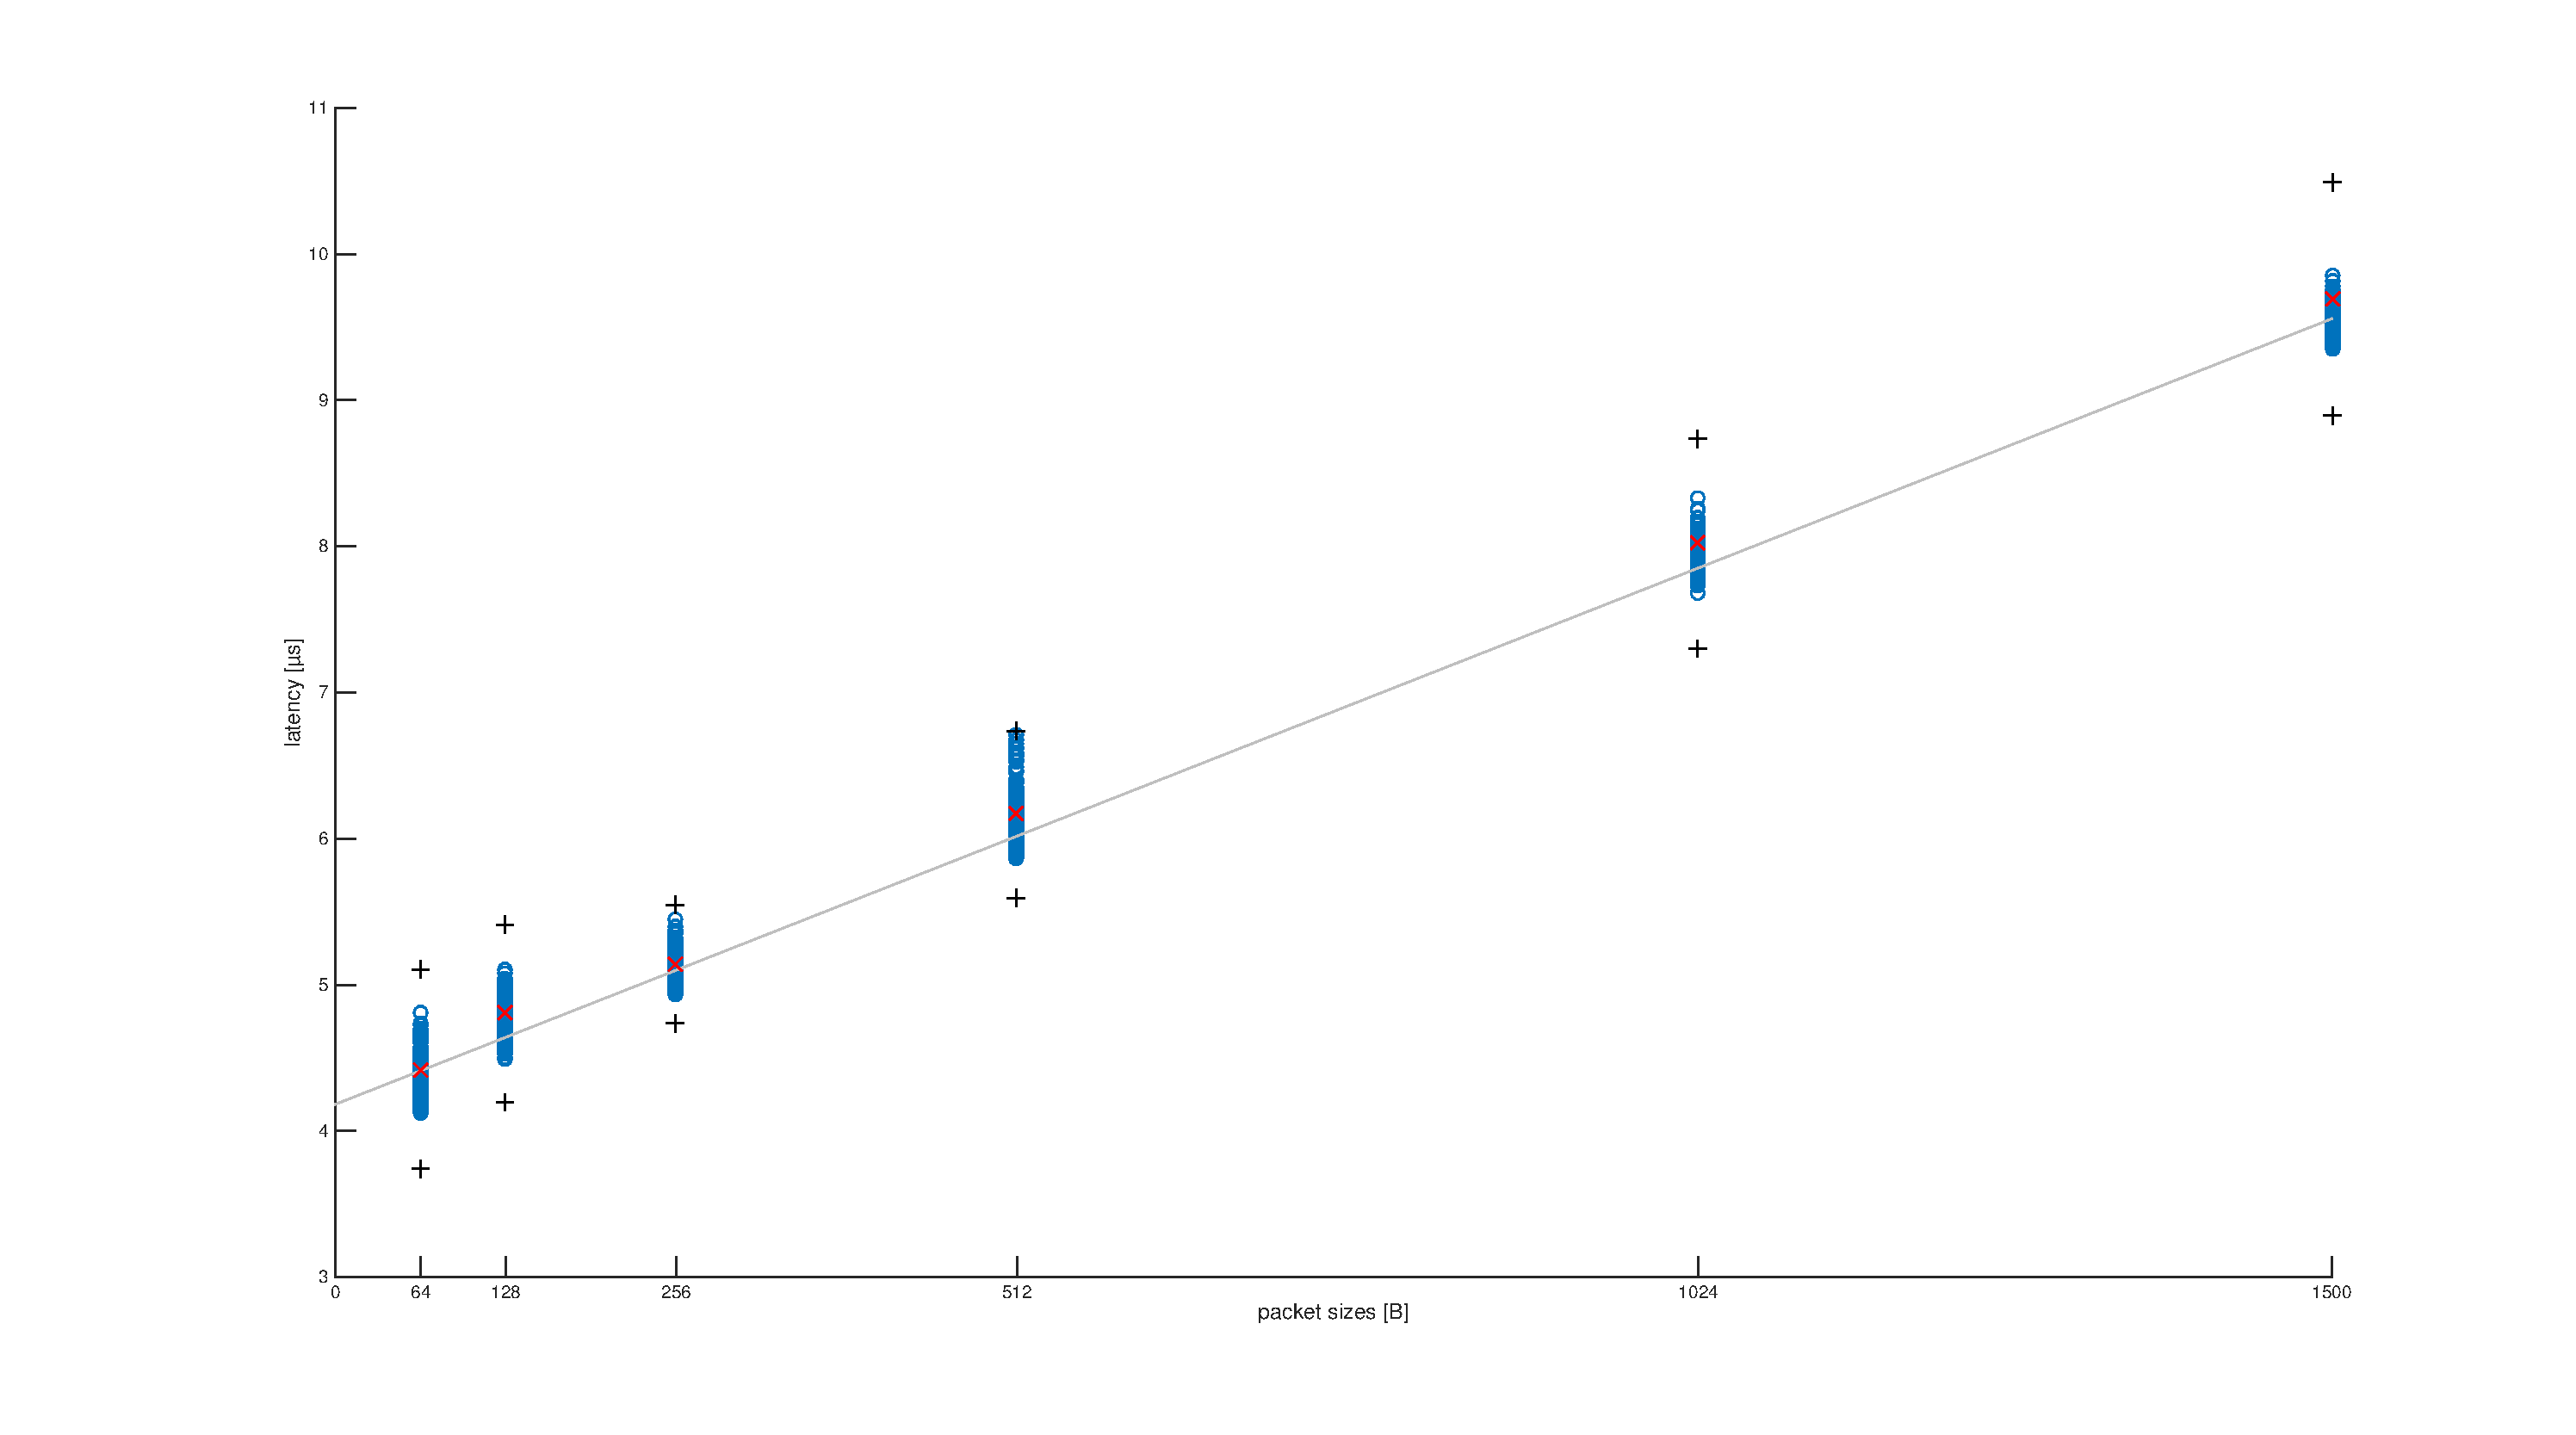
\includegraphics[width=\textwidth]{images/comm-latency.pdf}
    \caption{Latency of the input and output phase of the CN6880 unit. Averages marked as red X, and the 99\% confidence intervals with +. The trendline is of equation.}
    \label{fig:comm-latency}
  \end{center}
\end{figure}
\todo[inline]{check the confint}
\todo[inline]{latency = a*packetsize + constant}

As shown in the Figure~\ref{fig:comm-latency}, the time spent in the input and output phase of the unit is linear regarding to the packet size. The variation of the data is relatively small, and all the measurements correspond to the values measured with the external traffic-generator.

\todo[inline]{the following needs to be explained somewhere with the other fastpath stuff.}
\todo[inline]{Regardless of the packet size, the size of the work queue entry handled by the input/output units is the same.}
\todo[inline]{Also, the forward/swap code is constant in terms of packet size.}
\todo[inline]{Only operation that is dependent on the packet size is the copy from input to L2/RAM and from L2/RAM to output unit.}

As explained earlier\todo{actually explain this}, the only packet size dependent operations in the input/output phase are the  memory transfers between the memory (L2/RAM) and PKI or PKO.

We can not make a distinction between the input and output phase.
In our model, we will adjust the input/output phase amount so that they consume the PKI and PKO units for the amount that corresponds the constant term of equation \ref{eq:1}. The variable (non-constant) term is caused by the memory copies in the input/output phases, and are proportional to the packet size.

\subsection{Memory Delays}
\label{sec:memory-delays}

Memory delays were measured using Multi-core Processor Architecture and Communication (MPAC) benchmarking library. \cite{cite} Both, latency and throughput, were measured using for different dataset sizes and number of threads.

\begin{figure}[]
  \begin{center}
    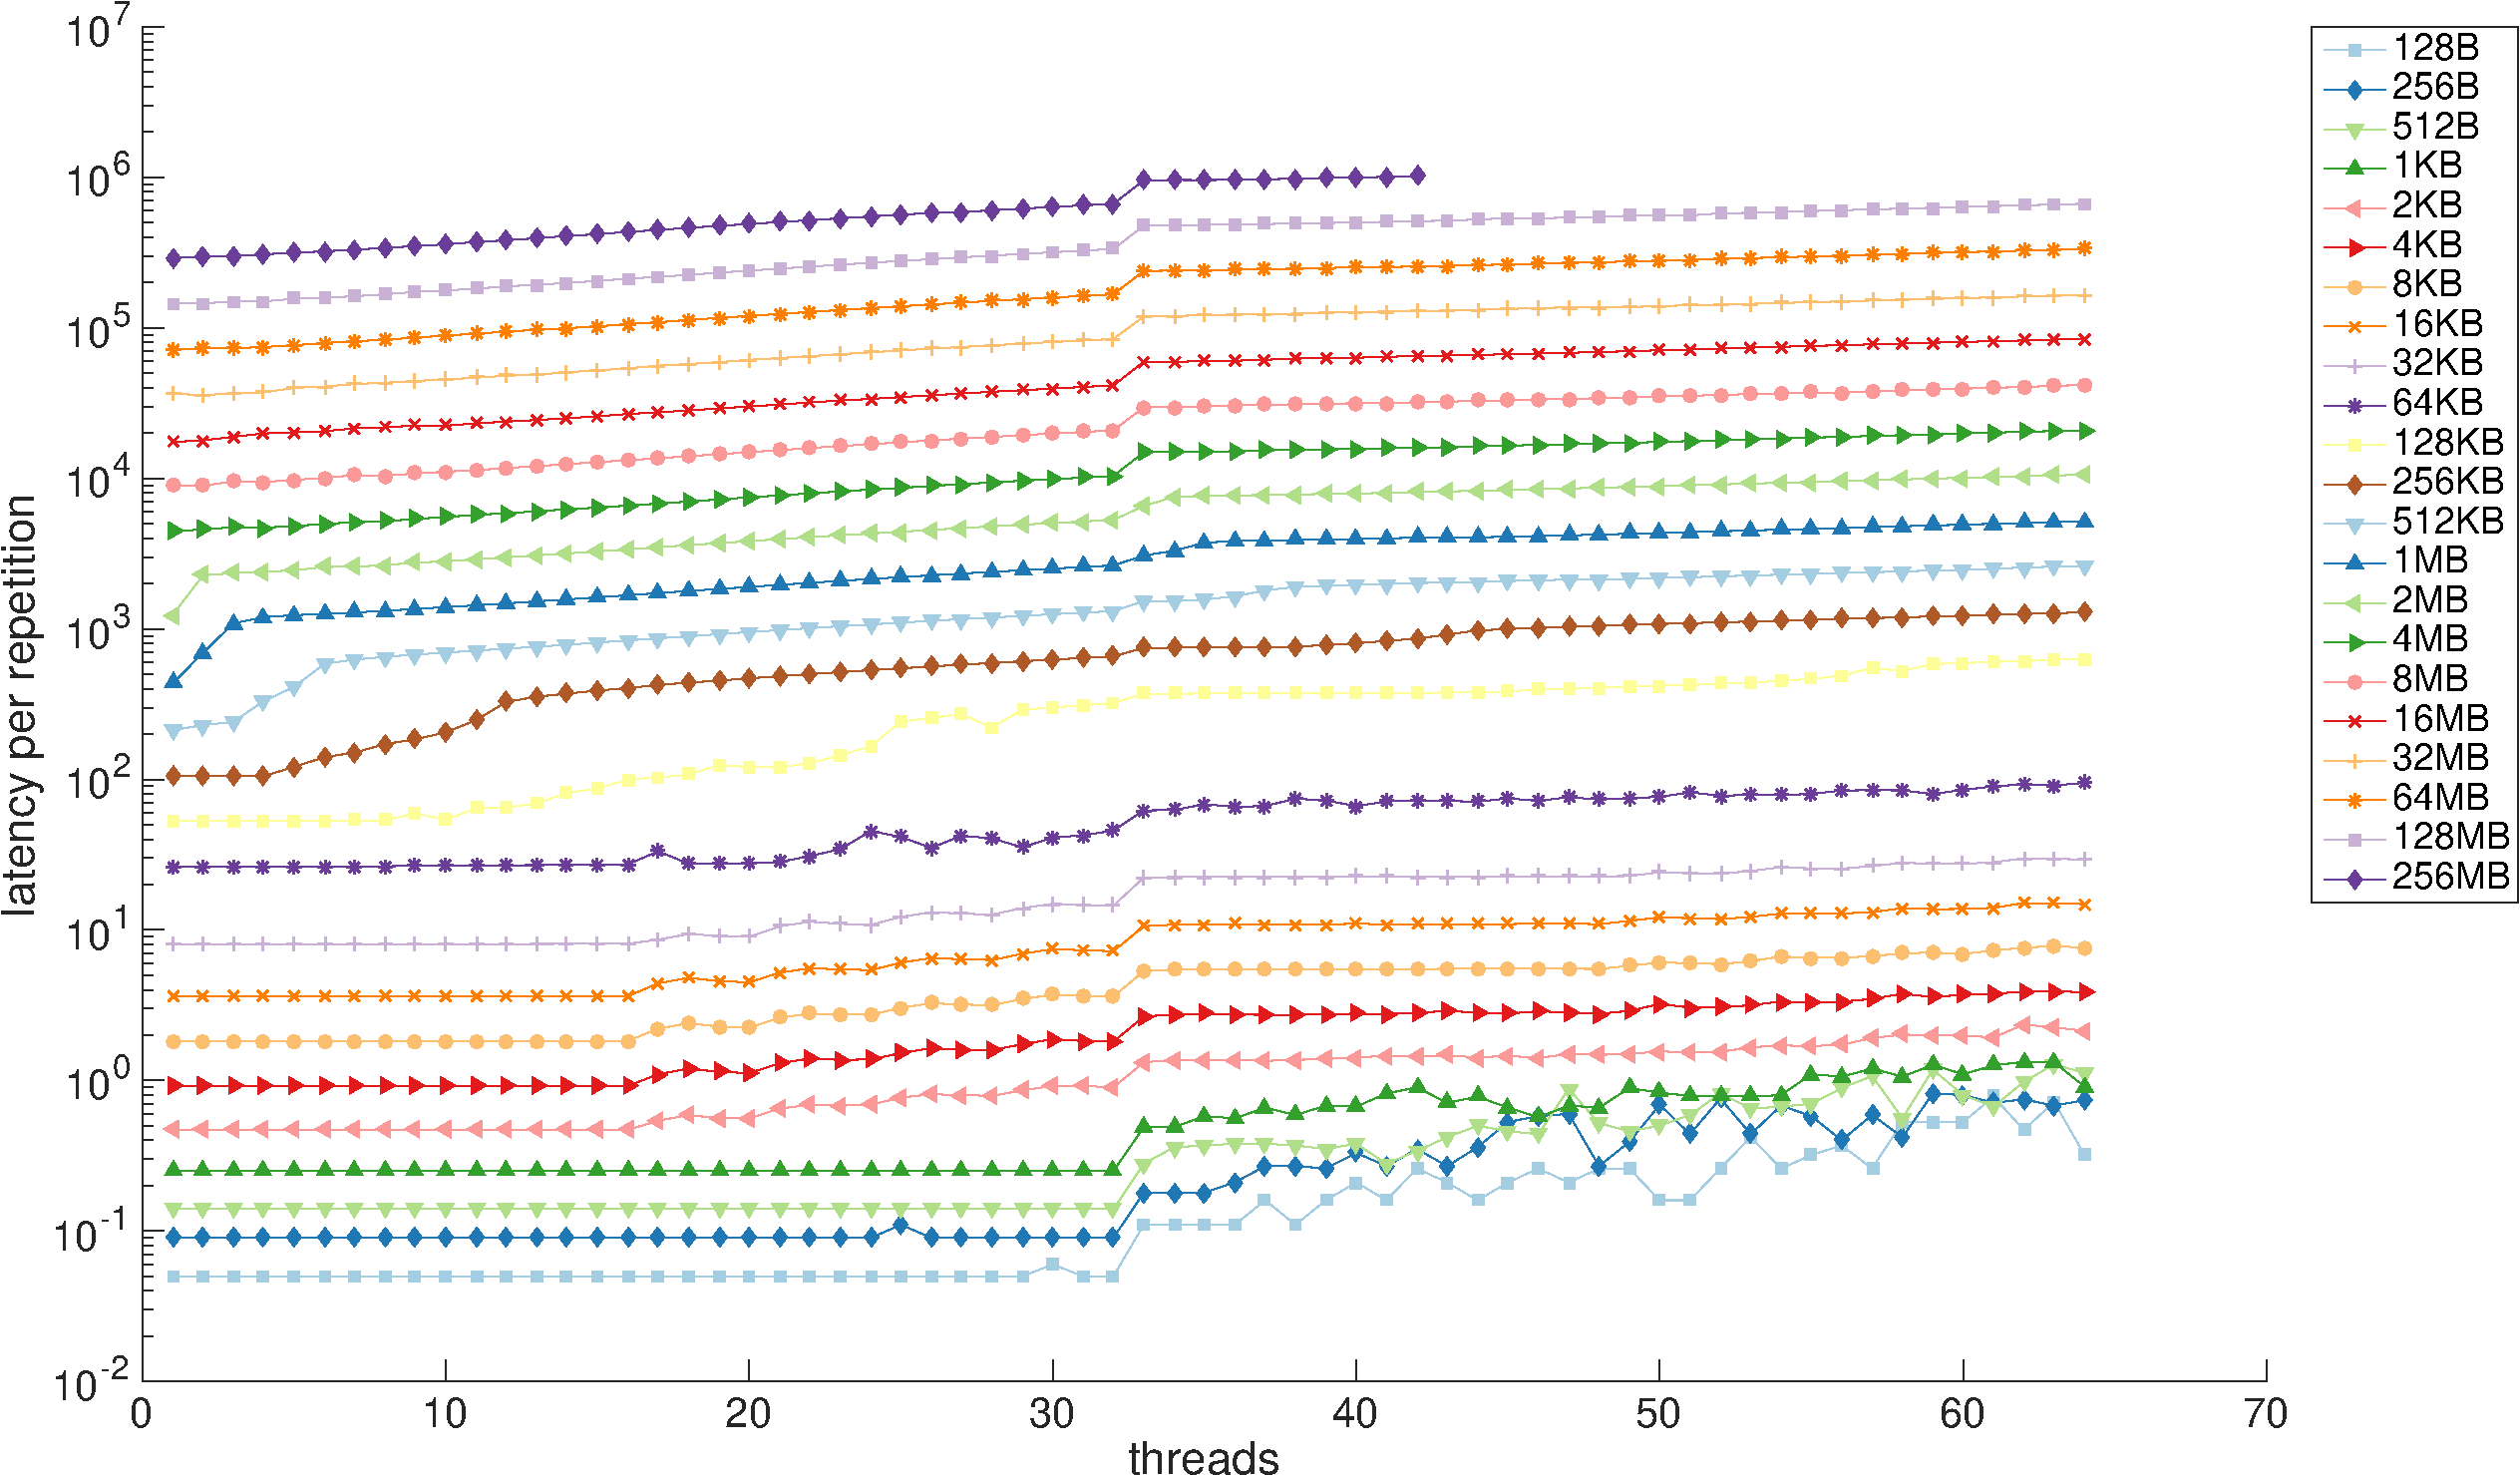
\includegraphics[width=\textwidth]{images/mem-latency.pdf}
    \caption{Memory latencies of the CN6880, measured by MPAC.}
    \label{fig:mem-latency}
  \end{center}
\end{figure}

\todo[inline]{logarithmic Y-scale}
\todo[inline]{explain the figure}

\begin{figure}[]
  \begin{center}
    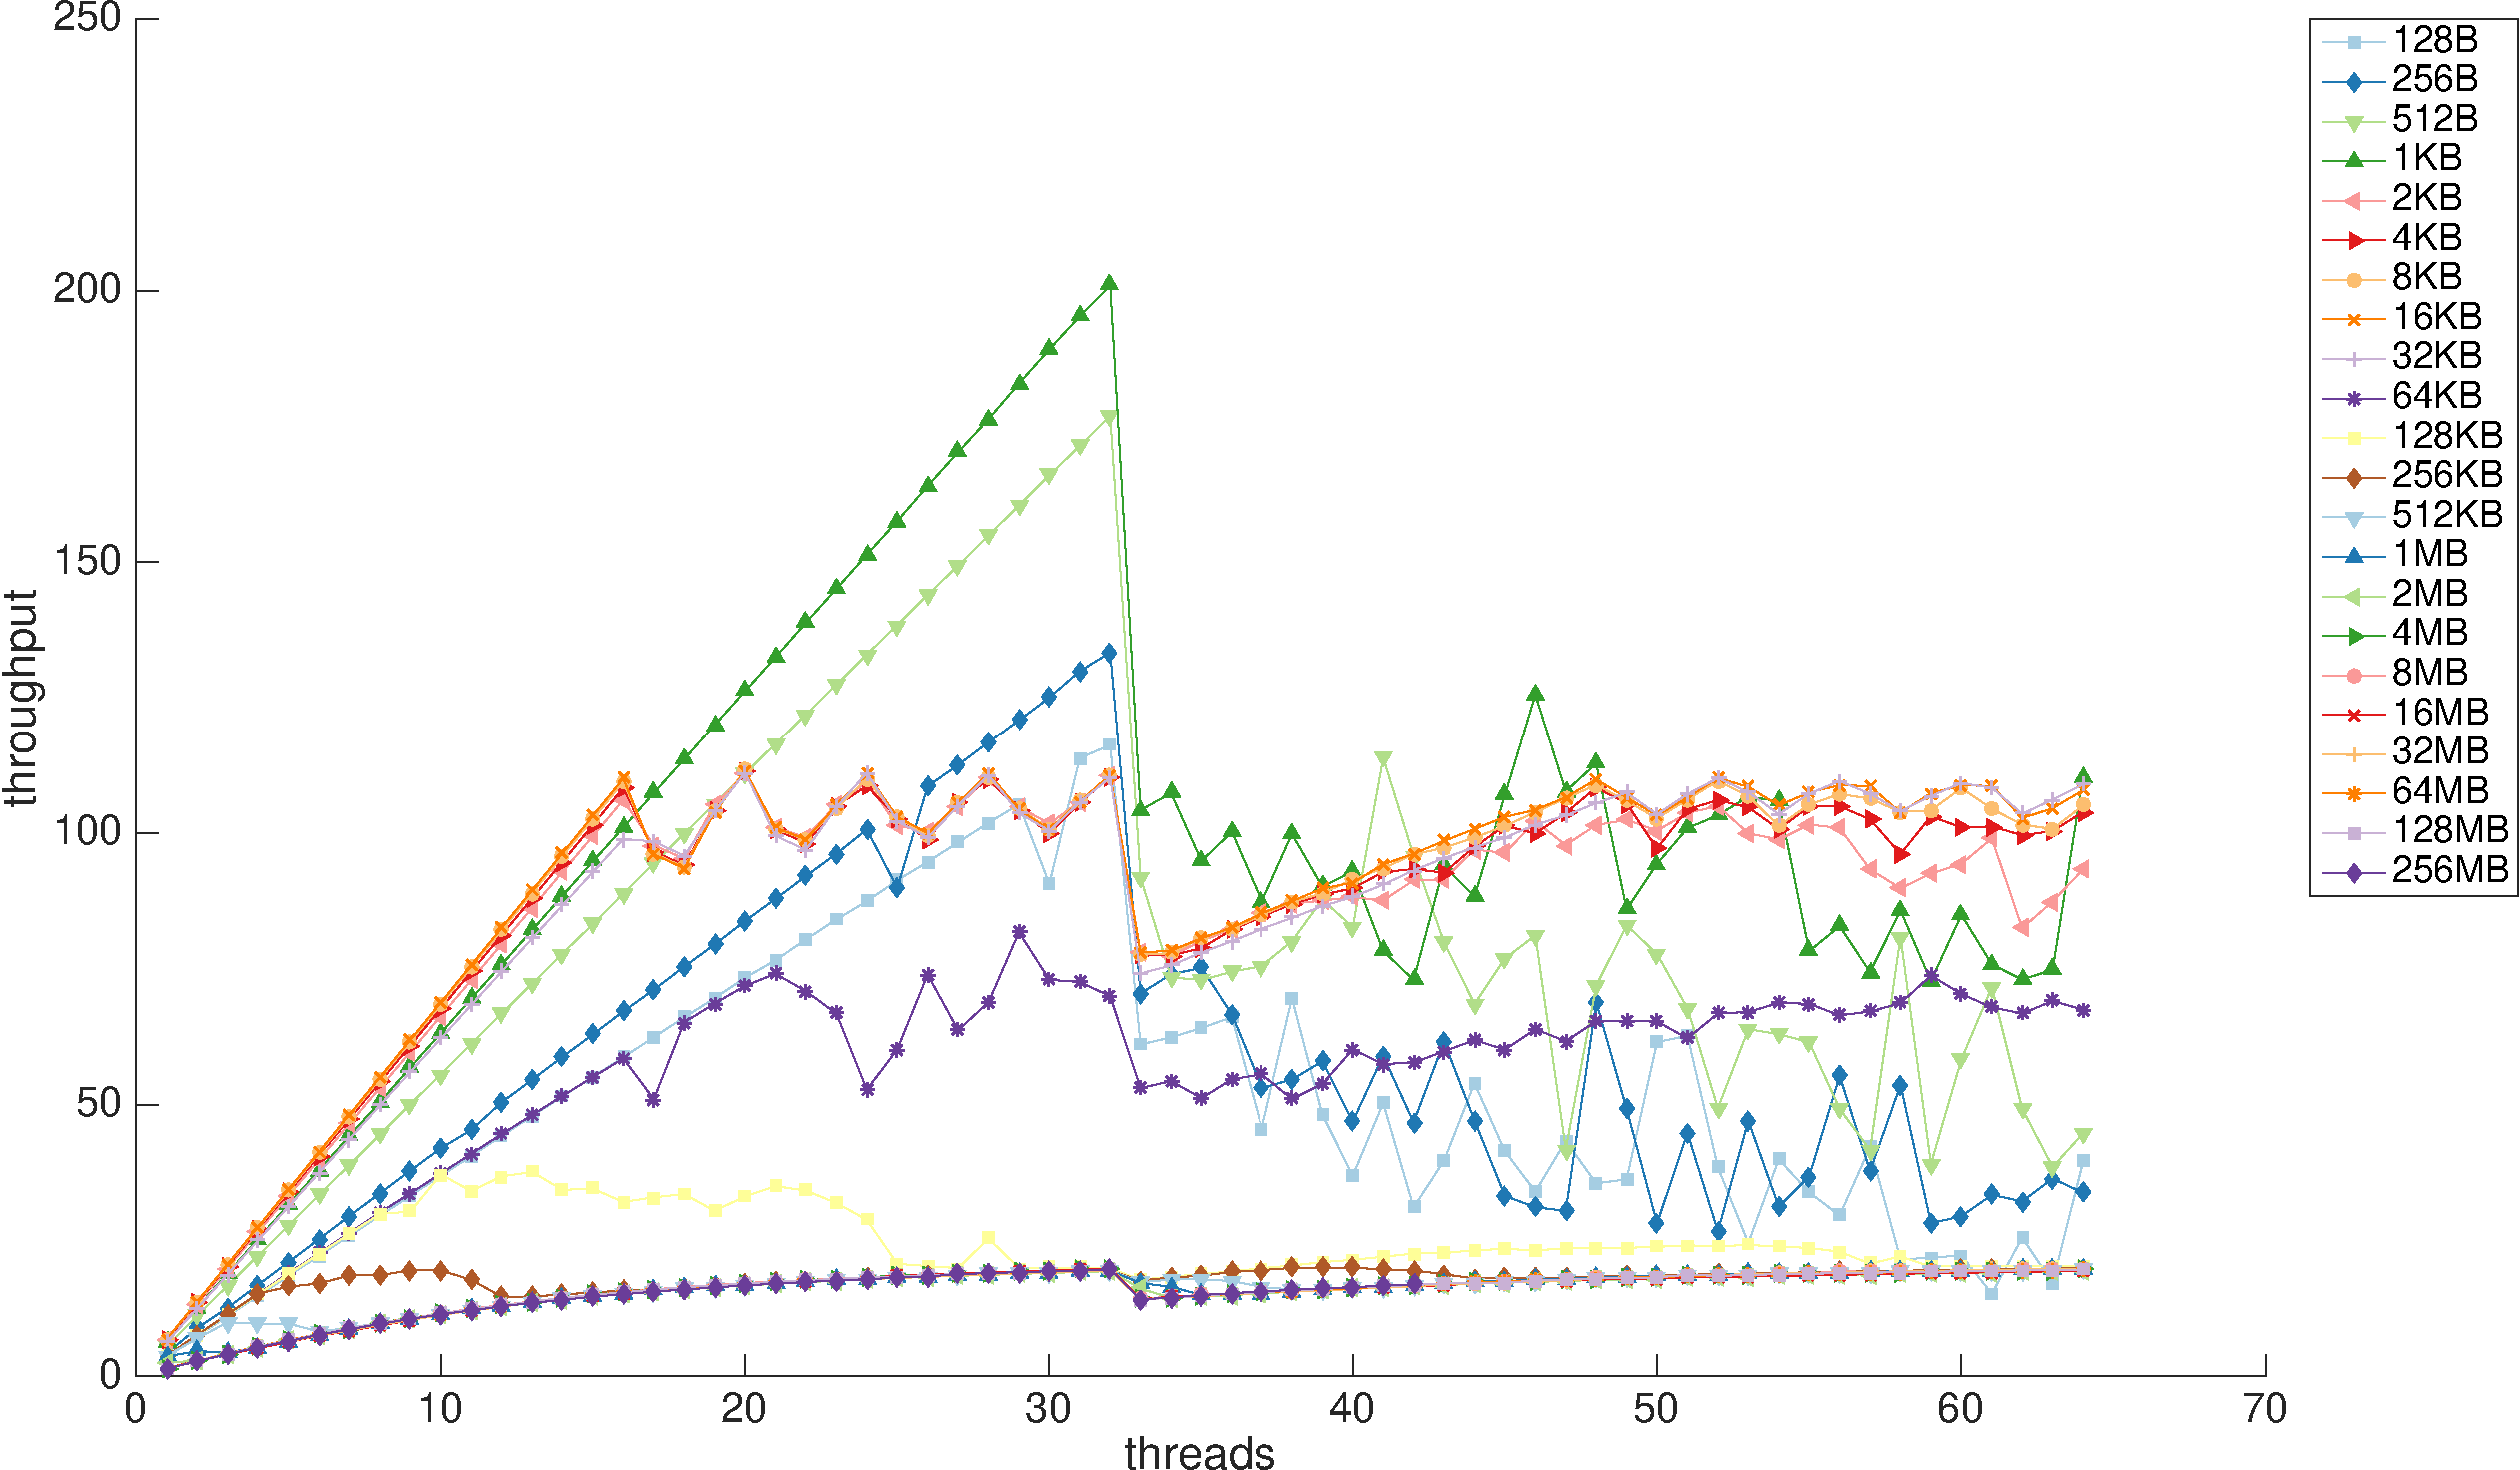
\includegraphics[width=\textwidth]{images/mem-throughput.pdf}
    \caption{Memory throughput of the CN6880, measure by MPAC.}
    \label{fig:mem-throughput}
  \end{center}
\end{figure}

\todo[inline]{explain the figure}

\section{Simulation Model}
\label{sec:simulation-model}

We created a high level simulation model of the Cavium OCTEON II CN6880 network processing unit with Performance Simulation Environment. As our interests are mainly in the applications' effect on the packet throughput and latency, we will not model the specific details of the hardware components. Figure \ref{fig:full-model} shows a layered representation of the main components of the final model: workload, hardware, and software.

\begin{figure}[]
  \begin{center}
    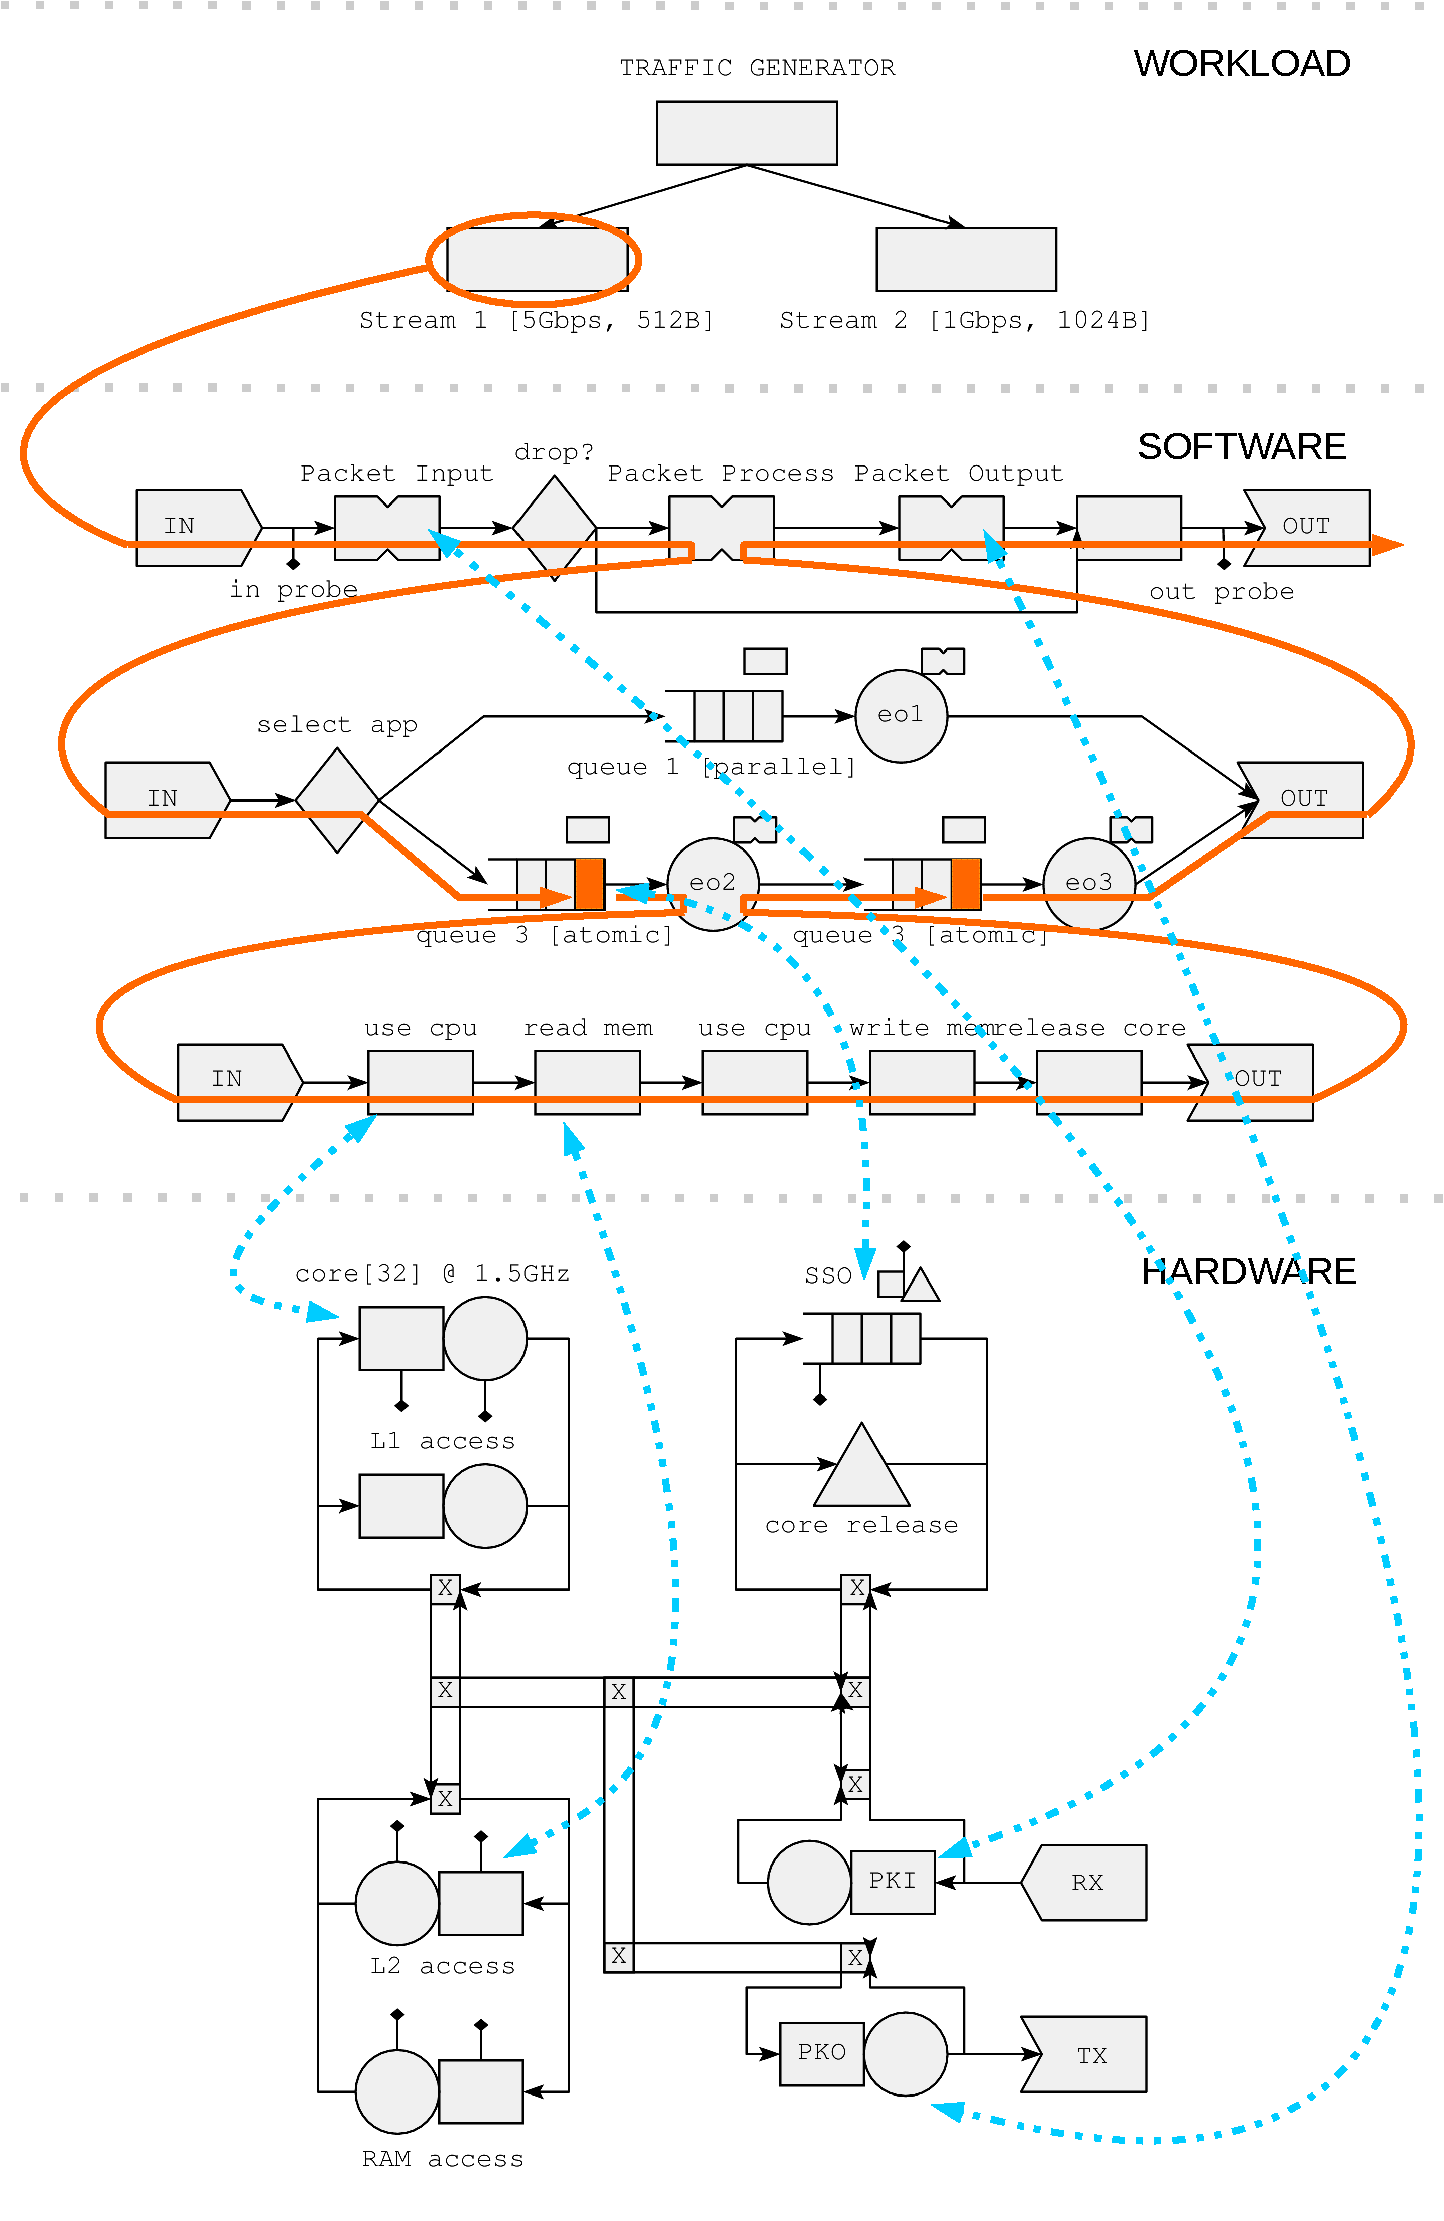
\includegraphics[width=\textwidth]{images/fullmodel-crop.pdf}
    \caption{Graphical presentation of the OCTEON II CN6880 PSE model. The workload model (top) generates network packets, which then flow through the software model (middle), consuming the hardware resources (bottom). The orange arrows represent an example of a packet's path through the software model, and the blue arrows the resource usage at each software model node.}
    \label{fig:full-model}
  \end{center}
\end{figure}

The workload model, at the top of the picture, consists of two packet streams. The TRAFFIC GENERATOR node activates the two stream nodes, which again generate packets that enter the software layer. The workload nodes contain parameters, such as the application id's, that are used to control the packet flows in the software model.

% has a lifetime of 0.5 seconds, and it triggers the streams with interval drawn from a uniform distribution with parameters 0.00005 and 0.00015. The streams have lifetime of 0.0004 seconds, and interval drawn from a lognormal distribution. The packet sizes of the streams are defined with the size attribute. Both of the streams also specify an appId attribute that is used to define the processing application in the software model. The packets from both streams enter the IN node of the top level software model.

The software model is divided into several submodels. The top software level model consists of packet input, packet processing and packet output submodels. The submodel view of the packet input and packet output are omitted from the picture for the sake of simplicity, as in both of these phases, the core and memory usage is linearly dependent on the packet size with additional Gaussian noise. In the input phase, the packet consumes specific amount of core cycles for the header processing, and copies the packet header and the packet data to the memory. Packet output node copies the packet from the memory, and consumes certain amount of clock cycles for the packet checksum calculations.

The packet processing submodel is presented in the middle software layer. The select app node forwards each of the packets to one of the two packet processing application, based on the application id attribute defined in the workload model. The queue nodes represent the core scheduling done by the SSO hardware unit. The packets arriving in the upper application have priority of 1, and they can be processed in parallel. In the application below, there are 2 atomic queues with priority 3. When the packet receives the passive resource from SSO, it can enter the actual processing application, called execution object (eo). The execution objects are submodels that consume core cycles and memory similarly to the packet input and packet output submodels presented above. The SSO/core passive resource is released inside each execution object.

The hardware model is a simple one level model containing no submodels. In the bottom left hand corner, there are PKI and PKO devices providing processor cycles for the packet input and packet output phases. The only passive resource node, SSO, provides core access resources, that can be released with the core release node. The application cores are shown in the top left corner of the hardware layer. There are 32 cores, and a specific L1 cache access for each of them. The L2 and RAM memory resources provide the delay for reading and writing to memory.

The probes, attached to the SSO unit, the cores, and the memory nodes, are used to gather statistics from the execution. Each of the units have two probes, one to measure the resource usage, and the other to measures the queue for the corresponding resource. In this hardware model, the routing nodes (squares) and the edges connecting the resources do not have any functional meaning, but are used solely to mimic the graphical models of the CN6880 unit presented in~\cite{cavium:2010:fundamentals}.

\section{Modeling the Task Scheduler}
\label{sec:modeling-task-scheduler}

The Schedule/Synchronization/Order (SSO) unit has an important effect on the task throughput times, as it controls the order in which the task get service from the application cores. This section first describes the application nodes used to model the SSO unit, and then the actual plug-in functions used to implement the scheduling functionality on the hardware model level.

% The SSO unit assigns the tasks to the processing cores.

% SSO unit needs to have a global

% The SSO unit schedules the tasks for the cores based on the

% Modeling a task processing application

% Figure~\ref{fig:full-model} has two different task processing applications.

% Before the task can be processed, it must wait for the SSO to schedule it on the core.

% When modeling the applications on PSE, it is helpful to consider the flow from the task's perspective. When a task has passed the input processing, it is put into the SSO queue to wait to be scheduled on the application cores. Each time a core finishes its previous task, it requests for a new work from the SSO-unit, which then schedules a task based on the flow QoS priority and work group.

\subsection{Application Models}
\label{application-models}

Each packet processing application consists of two parts: the SSO queue node, and the actual processing. The software layer in Figure~\ref{fig:full-model} presents and example of two main applications. The second application is divided into two sub-applications. The parameters for the first application's queue and execution object are shown in the Listings~\ref{lst:queue-attributes} and ~\ref{lst:eo-attributes}, respectively.

\lstinputlisting[caption=The attributes of the SSO queue.,
                 label=lst:queue-attributes]{listings/queue-attributes.txt}

The first line in Listing~\ref{lst:queue-attributes} specifies the display title for the node, as shown in the Figure~\ref{fig:full-model}. The \emph{name} and \emph{type} attributes specify that the resource usage is passive, and the required resource provision entity is $core\_require$, i.e. the SSO. The parameters on lines 5-7 define the parameters that are used in the custom scheduling code on the hardware level. The \emph{$queue\_type$} value atomic specifies that two nodes entering the SSO from the same resource usage node, cannot be processed simultaneously. The \emph{$queue\_id$} is used to keep track of the tasks being processed, and \emph{$queue\_priority$} is used to globally prioritize tasks between the queues.

\lstinputlisting[caption=The attributes of execution object.,
                 label=lst:eo-attributes]{listings/eo-attributes.txt}

nThe execution object node parameters are shown in the Listing~\ref{lst:eo-attributes}. It is a simple submodel node. It specifies the display title, and the name of the submodel to be used. The \emph{file} attribute specifies the file that defines the submodel. Note that, each execution object submodel needs to release the SSO/core resource, as shown in the Figure~\ref{fig:full-model}.

\subsection{Custom Scheduler Functions}
\label{sec:custom-scheduler-functions}

% Because the tasks processing in CN6880 is done in run-to-completion manner, the SSO unit is modeled as a passive resource. Each time when a tasks is entering a processing application, it must acquire the passive SSO resource. The amount of available passive SSO resources are equal to the processing cores in the system, and a task cannot use processing core without holding the SSO resource.

% The SSO scheduling is done in the SSO node presented in the hardware level in Figure~\ref{fig:full-model}. The actual scheduler function is written as a plug-in code, using the interface provided by PSE. The custom scheduling in PSE requires two functions, which are written in C-code: the selection function, and the reserve function. Each time a task enters a resource usage node in the task graph, the reserve function is called. The reserve function either

To model the SSO unit, a custom scheduling functions are required. PSE enables fully customizable resource scheduling through its plug-in interface. The actual scheduling functions are written in C-code, and the resource node parameters are changed to use these functions. The parameters of the SSO node used in the example model are presented in the Listing~\ref{lst:RNS-attributes}.

\lstinputlisting[caption=The attributes of the SSO node to determine the custom scheduler.,
                 label=lst:RNS-attributes]{listings/SSO-attributes.txt}

The first three lines specify the node title, name, and capacity. The capacity is set to the amount of available processing cores, meaning that no more than 32 tasks can be processed simultaneously. The \emph{discipline} parameter \mbox{CUSTOM}, on line 5, specifies that a custom scheduler is used instead of the built-in scheduling functions. The \emph{file} parameter specifies the path of the C header file that declares the scheduling functions. The \emph{$select\_function$} and the \emph{$reserve\_function$} parameters specify the two functions that are required to implement the scheduling logic.

The reserve function is called each time a task enters a resource usage node in the resource usage model, and it determines whether the task can immediately be served, or if it has to wait for the service. If the task can be processed immediately, it is inserted to the processing queue of the resource, and to the waiting queue otherwise. If the task gets put to the waiting queue, the reserve function also needs to reorder the queue.

Listing~\ref{lst:CUSTOM_reserve} describes the reserve function used to model the SSO. The function takes four input arguments: \emph{r} contains the data of the resource being reserved; \emph{queue} is a pointer whose value is assigned either to the processing queue or the waiting queue; \emph{position} is a pointer, whose value is assigned to the position in the queue; \emph{$new\_client$} holds the parameters, defined in the workload and resource usage models, of the new task.

\lstinputlisting[caption=The $CUSTOM\_reserve$ function for SSO.,
                 label=lst:CUSTOM_reserve]{listings/CUSTOM_reserve.c}

On the lines 11-39\todo{check the lines if the code changes!}, the reserve function attempts to place the task in the processing queue. The if-statement, on line 11, checks if the resource capacity is full. If there are available cores, then the processing conditions are checked, by going through all the cores, as shown in the for-loop on lines 21-32. If the new task's flow is marked atomic (in the reserve node in resource usage graph), and another task from the same flow is being processed on one of the cores (if-condition on lines 25-26), then the for-loop breaks, and the task gets set to the waiting queue. If a core is not processing, and the flow's coremask permits processing on the core (if-condition on line 31), we assign core's index to variable \emph{j}. Finally, if there is available core (\emph{j} is smaller or equal than the resource capacity) and none of the tasks from the same atomic flow are being processed, we set the queue to point to the resource's processing queue, and the position to the variable \emph{j}, and return.

If the processing conditions are not met, i.e. the execution goes past the if-block, then the task is set into the waiting queue. Line 43 assigns the \emph{queue} to point to the waiting queue of the resource. The for-loop on lines 46-48 finds the first task with larger priority, at index \emph{i}, and the for-loop on lines 51-53 moves all the higher priority tasks one step further on the queue. Finally the index \emph{i} is assigned to \emph{position}, and the function returns.

Each time a core ends a processing of a task, a new task is selected for the processing, using the the custom select function. Listing~\ref{lst:CUSTOM_select} shows the code used for the select function to model the SSO.

\lstinputlisting[caption=The $CUSTOM\_select$ function for SSO.,
                 label=lst:CUSTOM_select]{listings/CUSTOM_select.c}

$CUSTOM\_select$ takes the resource \emph{r}, and the index of the released core \emph{$release\_index$} as an input. The outer for-loop, starting at line 7, goes through all the tasks in the waiting queue, and finds the first task that satisfies the processing constraints, similarily as the reserve function. Line 10 checks if the waiting task's coremask allows the task to be processed on the core. If the waiting task's flow is atomic (line 12), we need to go through all the processing cores to check that there is no task being processed from the same flow (lines 18-24). If the task was not atomic, or no tasks from the same flow were being processed, the function returns the index of the task in the waiting queue. Otherwise we move to the next waiting task and repeat. If no task from the waiting queue can be scheduled, the function returns $RNS\_LARGE$. The RNS automatically moves the clients when it removes the task from the waiting queue.

%%% Local Variables:
%%% mode: latex
%%% TeX-master: "thesis-hartikainen"
%%% End:
